\documentclass[12pt]{article}

% packages
\usepackage{geometry}
\usepackage{amsmath}
\usepackage{amsfonts}
\usepackage{enumitem}
\usepackage{graphicx}

\usepackage[numbered,framed]{matlab-prettifier}

\newcommand{\Problem}[1]{\subsection*{Problem #1}}
\newcommand{\Q}[1]{\subsubsection*{Q.#1}}
\newcommand{\union}[1]{\underset{#1}{\cup} }
\newcommand{\bigunion}[1]{\underset{#1}{\bigcup} \, }
\newcommand{\inter}[1]{\underset{#1}{\cap} }
\newcommand{\biginter}[1]{\underset{#1}{\bigcap} }

\newcommand{\minimize}[3]{\optimize{#1}{#2}{#3}{min}}
\newcommand{\maximize}[3]{\optimize{#1}{#2}{#3}{max}}

\DeclareMathOperator{\cov}{cov}
\DeclareMathOperator{\var}{var}


% parameters
\geometry{hmargin=1.5cm,vmargin=1.5cm}
\title{ORF523 - Problem Set 1}
\author{Bachir EL KHADIR }

\begin{document}
\maketitle

\Problem{1}

\Q{1}

\begin{enumerate}
\item Let $\lambda$ be an eigen value of $A^TA$ corresponding to an eigen vector $u \ne 0$, then $0 \le ||Au||^2 = u^TA^TAu = \lambda ||u||^2$, therefore $\lambda > 0$.
\item Let $\lambda$ be an eigen value of $A$ corresponding to an eigen vector $u$, the $A^TAu = A(Au) = \lambda^2 u$, so $\lambda^2$ is an eigen value of $A^TA$. Since $A$ has $n$ eigen values (accounting for multplicity), the eigen values of $A^TA$ are exactly the squares of the eigen values of $A$, and therefore the singular values of $A$ are the absolute values of the eigen values of $A$.

\item
  $$u_i^Tu_j = u_i^T\frac{A^TAu_j}{\lambda_j} = \frac{u_i^TA^TA}{\lambda_j}u_j$$
  Since $\lambda_i \ne \lambda_j$, $u_i^Tu_j = 0$
\end{enumerate}

\Q{2}
\begin{itemize}
\item The $L_2$ norm for vectors is unitarly invariant:
  Let $O$ unitary matrix and $X$ a vector, then $||OX||^2  = X^TO^TOX = X^TX = ||X||^2$.
\item Since $O$ is invertible, the application $S \rightarrow S, X \rightarrow OX$, where $S$ is the $L_2$ sphere, is a bijection. So   $\{ x, ||x||_2 = 1\} = \{ Ox, ||x||_2 = 1\}$
\item The $L_2$ norm for matrices is unitarly invariant.
  If $A$ a matrix, then $||AO|| = \max_{||x||_2 = 1} ||AOx|| = \max_{||Ox||_2 = 1} ||AOx|| = \max_{||y||_2 = 1} ||Ay|| = ||A||$ and
  $||OA|| = \max_{||x||_2 = 1} ||OAx|| = \max_{||x||_2 = 1} ||Ax|| = ||A||$.
\item
  Let $B$ be a matrix of rank at most $k$.
  $||A - B|| = ||U(\Sigma - U^TBV)V^T|| = ||\Sigma - U^TBV||$
  Let $U'\Sigma'V'$ be the SVD of $B$, by a similar argument: $||A - B|| = ||\Sigma - \Sigma'||$.
  
  $rank(B) = rank(\Sigma') \le k$, so $\Sigma'$ can be written as $\Sigma'^{(k)} = diag(\sigma_1', \ldots, \sigma'_k, 0 \ldots )$.
  $||A - B|| = \sqrt{\sum_{i = 1 ... k} (\sigma_i - \sigma'_i)^2 + \sum_{i = k+1 \ldots n} \sigma_i^2}
  = \sqrt{\sum_{i = 1 ... k} (\sigma_i - \sigma'_i)^2 + ||A - A^{(k)}||^2} \ge ||A - A^{(k)}||$,
  Since $rank(A^{(k)}) = k$ we have proved the result.
\end{itemize}

\Q{3}
\begin{enumerate}
\item
  \[
    \begin{array}{c|c}
      k & ||A - A_{(k)}||_F \\
      \hline
      25&51.5669\\
      50&31.7256\\
      100&18.2247\\
      200&10.0059\\
    \end{array}
  \]

 \item To store $A^{(k)}$ we need only to store $\Sigma^{(k)}$ ($k$ parameters), $U^{(k)}, V^{(k)}$ (each of them has only at most $k$ column not set to zero, so they take $nk + mk$), while $A$ takes $nm$ numbers to store.
   In conclusion, we save ($nm - k(n+m+1)$).
   \begin{itemize}
   \item 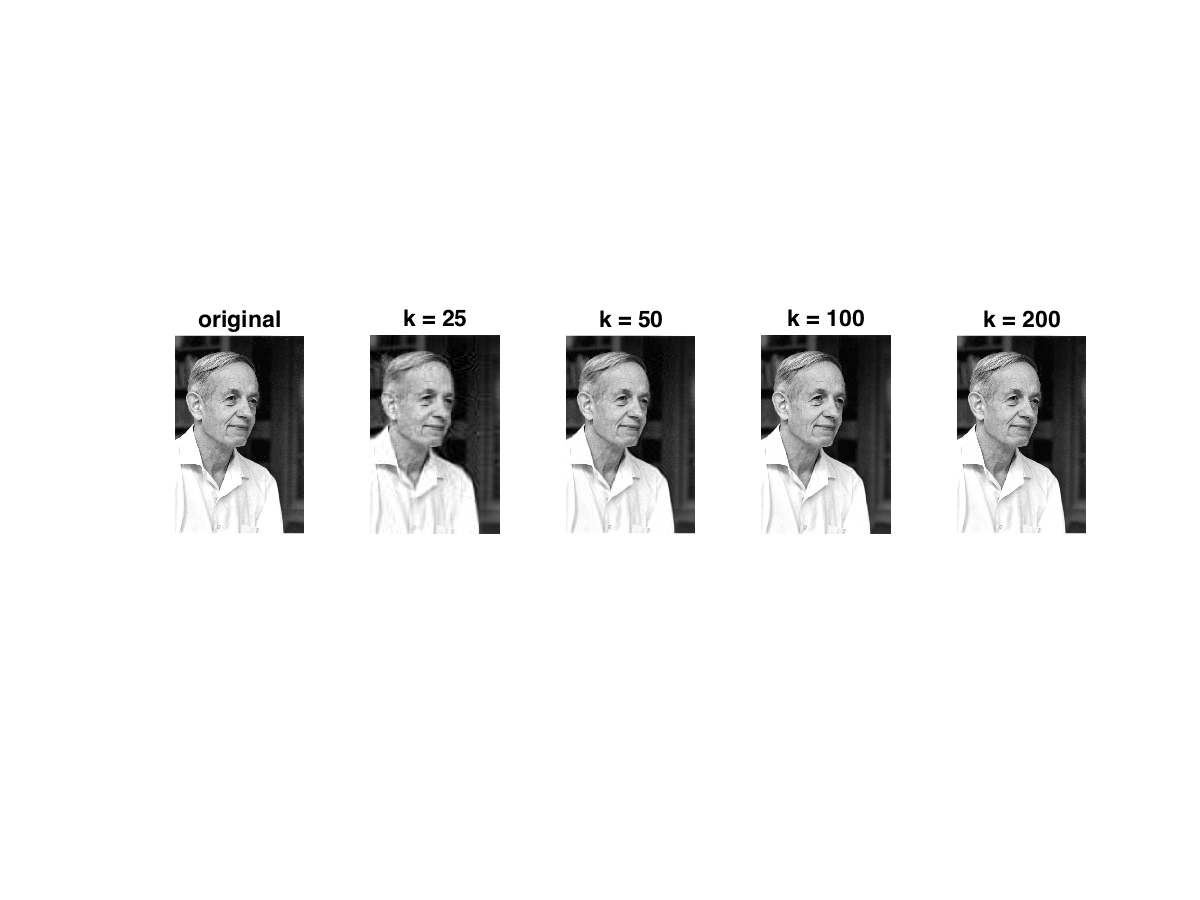
\includegraphics[scale=.25]{compressed.png}

   \item 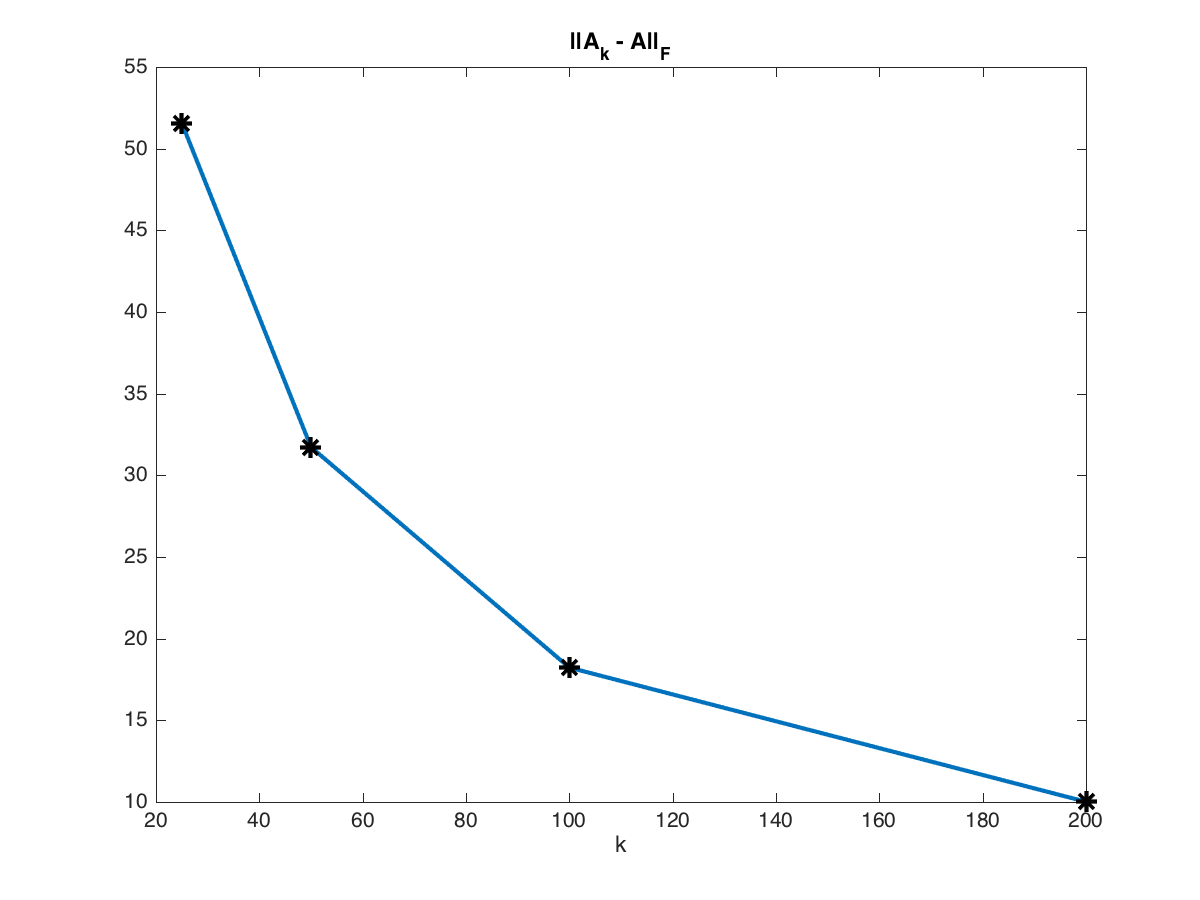
\includegraphics[scale=.25]{diffnorm.png}


   \item 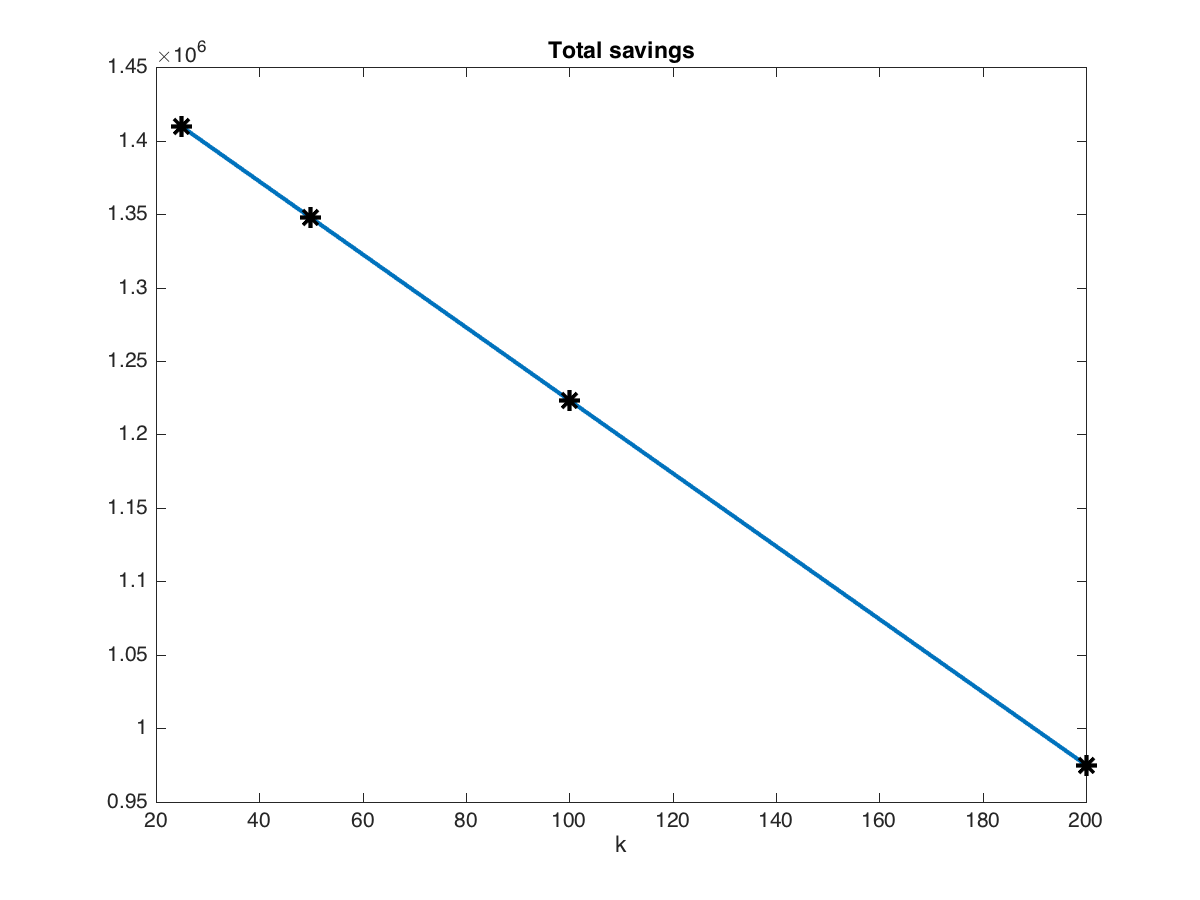
\includegraphics[scale=.25]{totalsavings.png}
   \end{itemize}
 \item Comparing the original and the compressed image for $k = 200$
   
   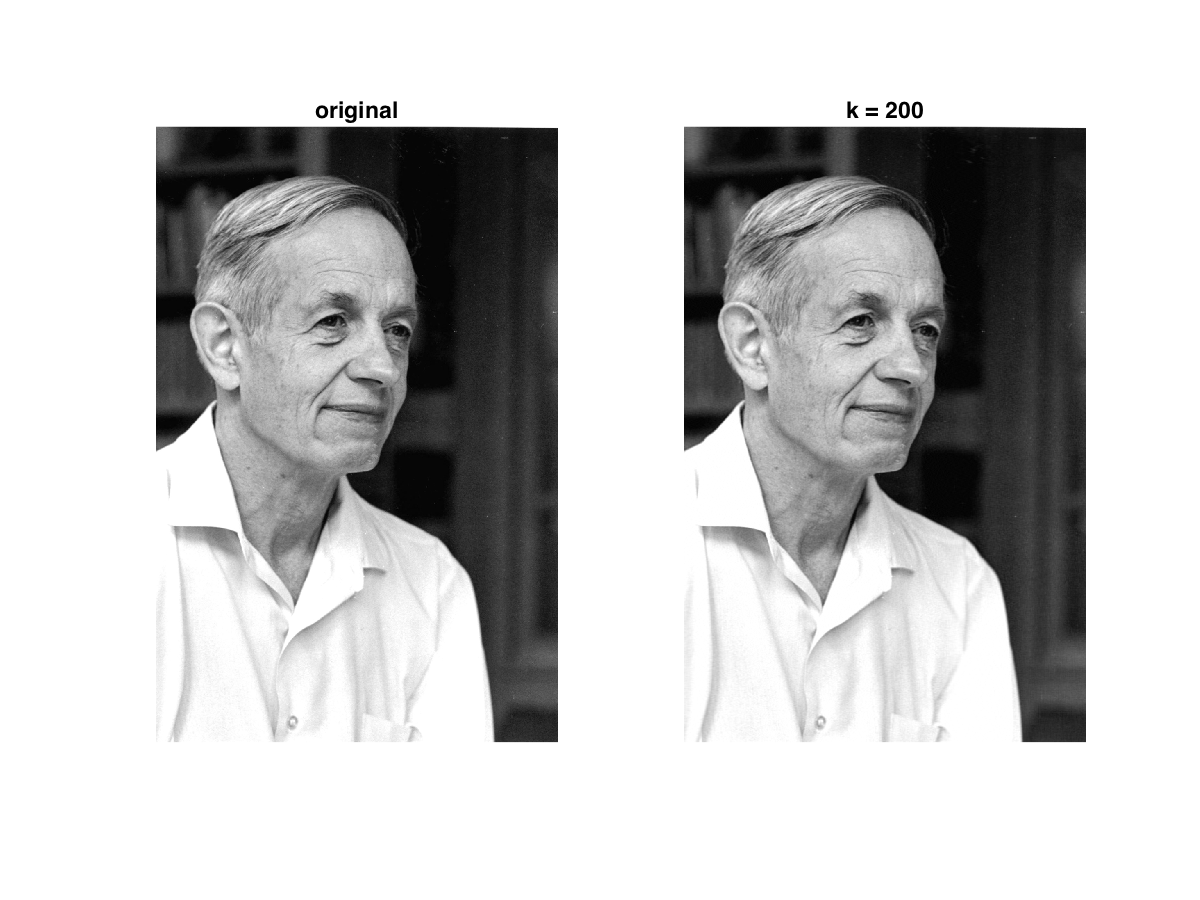
\includegraphics[scale=.25]{compare.png}
\end{enumerate}


\newpage
\subsubsection*{Code}
\lstinputlisting[style=Matlab-editor]{imageprocessing.m}
\newpage

\Problem{2}
\begin{enumerate}
\item
  Let $u = x_1 + x_2$, it is easy to verify that
  $f(x_1, x_2) = \underbrace{\frac {u^2}2 - 2u}_{g(u)} + \underbrace{- 2 x_2^2 + 3 x_2 + \frac13 x_2^3}_{h(x_2)} = g(u) + h(x_2)$

  Since this transformation is a diffeomorphisme, it preserves neighbourhoods, and therefore it preserves local minimizers/maximizers.

  A point $(u, x_2)$ is a local maximizer (resp. minimizer) of $g(u) + h(x_2)$ if and only if $u$ is a local maximizer (resp. minimizer) of $g$ and $x_2$ is local maximizer (resp. minimizer) of $h$.

  \begin{itemize}
  \item $g(u) = \frac12 (u-2)^2 - 2$ has one local(and global) minimum
    $u = 2$
  \item $h'(x_2) = x_2^2 - 4x_2 + 3 = (x_2 - 1)(x_2 - 3)$,
    $h''(x_2) = 2x_2 - 4$ 
  \end{itemize}
  The candidates are $x_2 = 1$ and $x_2 = 3$. Since $h''(1) = -2 < 0, h''(3) = 2 > 0$, $1$ is local maximum and $3$ is a local minimum.

  In conclusion, $(u, x_2) = (2, 1)$ is the only local optimizer (it is a local min) of $g(u) + h(x_2)$, and  $(x_1 = -3, x_2 = 1)$ is the only local optimzer (minimum) of $f$.

\item

  By Taylor expansion, since $f$ is a polynomial of order 2: $f(x) - f(\bar x) = \nabla f(\bar x)(x - \bar x) + \frac12 (x-\bar x)^T \nabla^2 f(x - \bar x) (x-\bar x)$

  \begin{enumerate}
  \item[a)]
  \begin{enumerate}
  \item[($\Rightarrow$)]
    Let $\bar x$ be a local min, then $\nabla f(\bar x) = 0$.
    If $\nabla^2 f$ is not positive semi-definite, let $d \in \mathbb{R}^n d^T\nabla f(\bar x) =: -\lambda < 0$, therefore $f(x + \alpha d) - f(x) = - \alpha^2 \lambda < 0$, and for any neighbourhood of $\bar x$, there exist $\alpha$ such that $\bar x + \alpha d$ is in that neighbourhood, and we have a contradiction.
  \item[($\Leftarrow$)]
    In this case: $f(x) - f(\bar x) = \frac12 (x-\bar x) \nabla^2 f(x - \bar x) \ge 0$, which proves that $\bar x$ is local min.
  \end{enumerate}

  \item[b)]
  \begin{enumerate}
  \item[($\Rightarrow$)]
    In this case: $f(x) - f(\bar x) = \frac12 (x-\bar x) \nabla^2 f(x - \bar x) > 0$, which proves that $\bar x$ is strict local min.
  \item[($\Leftarrow$)]
    In this case: $f(x) - f(\bar x) = \frac12 (x-\bar x) \nabla^2 f(x - \bar x) > 0$, which proves that $\bar x$ is strict local min.
  \end{enumerate}
\end{enumerate}

  Counterexamples:
  $f: \mathbb R \rightarrow \mathbb R, x \rightarrow x^3$, $f'(0) = 0, f''(0) = 0$, but $0$ is not a local min.
  $f: \mathbb R \rightarrow \mathbb R, x \rightarrow x^4$, $f'(0) = 0, f''(0) = 0$, but $0$ is a strict local min.
\item using the chain rule: $g'(\alpha) = \frac{d}{||d||} \nabla f(x + \alpha \frac{d}{||d||})$, $g'(0) \frac{d}{||d||}\nabla f(x)$, using Cauchy-Shwarz, this scalar product is minimal/ maximal when $d$ and $\nabla f(x)$ are colinear.
\end{enumerate}

\Problem{3}
$Q > 0$, so it admist an eigenvalue decomposition and all the eigen values are positive, let $Q = U\Sigma U^T$ be that decomposition, with $\Sigma = diag(\sigma_1, \ldots, \sigma_n)$, and Let $\sqrt{\Sigma} =diag(\sqrt{\sigma_1}, \ldots, \sqrt{\sigma_n})$, then $Q = \underbrace{U\sqrt{\Sigma}U^T}_{\sqrt Q}U\sqrt{\Sigma}U^T = \sqrt{Q}^2$

$f(x) = \sqrt{ x^T\sqrt{Q}\sqrt{Q}x} = \sqrt{ ||\sqrt Q x||^2} = ||\sqrt Q x||$

\begin{enumerate}
\item f is a norm because:

  \begin{itemize}
  \item $$f(\lambda x) = \sqrt{(\lambda x)^TQ(\lambda x)} = \sqrt{\lambda^2} f(x) = |\lambda| f(x)$$
  \item
    $$f(x + y) = ||\sqrt{Q}x + \sqrt{Q}y|| \le ||\sqrt{Q}x|| + ||\sqrt{Q}y|| \le f(x)+ f(y)$$
  \item $$f(x) = 0 \iff \sqrt{Q}x = 0 \iff x = 0$$
  \end{itemize}
\item

  By Riesz Representation theorem, we indentify a vector $x$ with the linear form $y \rightarrow x^Ty$.
  Let $g$ be the dual norm of $f$, then
  \begin{align*}
    g(x) &= \sup_{y \ne 0} \frac{x^Ty}{f(y)}
    \\&= \sup_{u \ne 0} \frac{x^T\sqrt{Q}^{-1}u}{||u||} &(y \rightarrow u=\sqrt{Q}y \text{ is a bijection})
    \\&= \sup_{u \ne 0} x^T\sqrt{Q}^{-1}\frac{u}{||u||}
    \\&= x^T\sqrt{Q}^{-1}\frac{(\sqrt{Q}^{-1}x)}{||\sqrt{Q}^{-1}x||} &\text{(Cauchy shwarz)}
    \\&= \frac{x^TQ^{-1}x}{\sqrt{x^TQ^{-1}x}}
    \\ &= \sqrt{x^TQx^{-1}}
  \end{align*}

\item
  $A^TA \ge 0$, Let $U\Sigma U^T$ be an eigen value decomposition where $\Sigma = diag(\sigma_1, \ldots, \sigma_n)$, and $\sigma_1 \ge \ldots \ge \sigma_n \ge 0$.
  
  \begin{align*}
    ||A||_2 &= \sup_{||x||=1} x^T(A^TA)x
    \\&= \sup_{||x||=1} ||\sqrt{A^TA}x||
    \\&= ||\sqrt{A^TA}||_2
    \\&= ||\Sigma||_2 \\&= \sup_{||x||=1} x^T(\Sigma)x \\&= \sup_{||x||=1} \sum_i x_i^2 \sigma_i \le \sum_{i} x_i^2 \sigma_1 \\&= \sigma_1 \\&= ||\Sigma e_1||
  \end{align*}

  So $||A||_2 = \sigma_1 = \sqrt{\lambda_{\text{max}}(A^TA)}$

\end{enumerate}
\end{document}
















